\chapter[Идентификация линейных стохастических систем]{%
  Идентификация линейных \chapternewline%
  стохастических систем
}

Как отмечалось в разделе~\ref{ssec:state_criterion},
оптимальным решением задач идентификации линейного полустохастического объекта,
а также линейного стохастического объекта первого типа является классическая линейная регрессия,
обеспечивающая как оптимальное оценивание параметров математической модели объекта
(при заданных значениях входных переменных),
так и оптимальное прогнозирование наблюдений выходных переменных по наблюдениям входных переменных.

Относительно стохастического объекта второго типа следует отметить,
что области предпочтительного использования классического и симметричного критериев идентификации
определены недостаточно четко.
Данная глава посвящена выявлению условий предпочтительного использования этих критериев
для оценивания параметров стохастических объектов второго типа,
а также прогнозирования наблюдений их выхода по наблюдениям входа.

\section{Методы и алгоритмы идентификации}

\subsection{Метод симметричной аппроксимации}\label{ssec:linear_method_symmetric}

Метод симметричной аппроксимации минимизирует сумму перпендикулярных расстояний
от аппроксимирующей гиперплоскости до результатов наблюдений.
Это соответствует использованию симметричного критерия идентификации
(рисунок~\ref{fig:state_criteria_symmetric}):
\begin{equation*}
  \rho_{\text{с}} = \sum_i \rho_{\text{с}_i} \rightarrow \min.
\end{equation*}

Алгоритм расчета оценок параметров линейной функции регрессии
методом симметричной аппроксимации составлен на основе теоремы, доказанной в статье~\cite{mukha_2016}.

Рассматривается случайный вектор \( \overline{\xi}^{\text{Т}} = (\xi_1, \ldots, \xi_m ) \in E^m \)
в \( m \)-мерном Евклидовом пространстве \( E^m \) и отыскивается линейная
зависимость последних \( r \) компонент этого вектора от \( m - r \) первых компонент
(последние \( r \) компонент вектора \( \overline{\xi} \) рассматриваются как выходные
переменные некоторого объекта, а первые \( m - r \) компонент "--- как входные).
Предполагается, что имеются измерения \( \overline{x}_i, i = \overline{1, n} \)
вектора \( \overline{\xi} \) (а не пар измерений вход-выход).

Входными параметрами алгоритма являются:
\begin{enumerate}
\item \( X \) "--- \( (m \times n) \)-матрица измерений
  (выборка размера \( n \) из распределения случайного вектора \( \overline{\xi} \)),
  \( i \)-тый столбец матрицы \( X \) представляет собой \( i \)-е измерение случайного
  вектора \( \overline{\xi} \);
\item \( r \) "--- количество последних компонент вектора \( \overline{\xi} \),\
  рассматриваемых как выходные переменные объекта.
\end{enumerate}

Алгоритм расчета оценок параметров имеет следующий вид:
\begin{enumerate}
\item Рассчитываются выборочные моменты \( \hat{\overline{a}}_{\xi}, D_{\xi} \) случайного вектора \( \xi \):
  \begin{equation*}
    \hat{\overline{a}}_{\xi} = \dfrac{1}{n} \sum_{i=1}^n \overline{x}_i, \quad
    \hat{D}_{\xi} =
    \dfrac{1}{n}  \sum_{i=1}^n
    (\overline{x}_i - \hat{\overline{a}}_{\xi})
    (\overline{x}_i - \hat{\overline{a}}_{\xi})^T.
  \end{equation*}
\item Формируется матрица \( P \), состоящая из собственных векторов матрицы \( \hat{D}_{\xi} \),
  расположенных в порядке убывания соответствующих им собственных чисел.
\item Формируются матрица \( C \), состоящая из \( m-r \) первых столбцов
  матрицы собственных векторов \( P \).
\item Выполняется разбиение матриц \( C \), \( X \) и вектора \( \hat{\overline{a}} \) на блоки:
  \begin{equation*}
    C =
    \begin{pmatrix}
      C_{m-r} \\
      C_{r}
    \end{pmatrix}, \quad
    X =
    \begin{pmatrix}
      X_{m-r} \\
      X_{r}
    \end{pmatrix}, \quad
    \hat{\overline{a}} =
    \begin{pmatrix}
      \hat{\overline{a}}_{m-r} \\
      \hat{\overline{a}}_{r}
    \end{pmatrix}.
  \end{equation*}
  Таким образом, матрица \( C_{m-r} \)  содержит первые \( m-r \) строк матрицы \( C \),
  матрица \( C_{r} \)  содержит последние \( r \) строк матрицы \( C \),
  матрица \( X_{m-r} \) содержит первые \( m-r \) строк матрицы \( X \),
  матрица \( X_{r} \) содержит последние \( r \) строк матрицы \( X \),
  вектор-столбец \( \hat{\overline{a}}_{m-r} \) содержит первые \( m - r \) компонент
  вектор-столбца \( \hat{\overline{a}} \),
  а вектор-столбец \( \hat{\overline{a}}_{r} \) содержит последние \( r \) компонент
  вектор-столбца \( \hat{\overline{a}} \).
\item Рассчитывается векторы коэффициентов \( \overline{\alpha}, \overline{\beta} \)
  линейной аппроксимирующей зависимости
  \( X_r = \overline{\alpha} + \overline{\beta} X_{m-r}\)
  в соответствии с формулой
  \[ X_r = \hat{\overline{a}}_r + C_r (C_{m-r})^{-1} (X_{m-r} - \hat{\overline{a}}_{m-r}), \]
  то есть рассчитываются
  \begin{equation*}
    \begin{aligned}
      \overline{\beta} &= C_{r} (C_{m-r})^{-1}, \\
      \overline{\alpha} &= \hat{\overline{a}}_{r} - \overline{\beta} \; \hat{\overline{a}}_{m-r}.
    \end{aligned}
  \end{equation*}
\end{enumerate}

Результатом работы алгоритма являются \( \overline{\alpha}, \overline{\beta} \) с учетом того,
что аппроксимирующая гиперплоскость определяется формулой
\[ \overline{y} = \overline{\alpha} + \overline{\beta} \overline{x}, \]
где \( \overline{y} \) "--- \( r \)-мерный вектор выходных переменных, \\
\hspace*{7mm} \( \overline{x} \) "--- (\( m - r \))-мерный вектор входных переменных.

\subsection{Классический метод наименьших квадратов}\label{ssec:linear_method_classic}

Классический метод наименьших квадратов ставит своей целью минимизировать сумму
вертикальных расстояний от аппроксимирующей гиперплоскости до результатов наблюдений.
Это соответствует использованию классического критерия идентификации
(рисунок~\ref{fig:state_criteria_classic}):
\begin{equation*}
  \rho_{\text{к}} = \sum_i \rho_{\text{к}_i} \rightarrow \min.
\end{equation*}

Значения параметров классической линейной регрессии
\( \overline{y} = \overline{\alpha} + \overline{\beta} \overline{x} \)
с учетом обозначений и исходных данных, принятых в подразделе~\ref{ssec:linear_method_symmetric},
определяются формулами
\begin{equation*}
  \begin{aligned}
    \overline{\beta} &= R_{yx} D^{-1}_{x}, \\
    \overline{\alpha} &= \hat{\overline{a}}_{r} - \overline{\beta} \; \hat{\overline{a}}_{m-r},
  \end{aligned}
\end{equation*}
где \( D_x \) "--- \( (m-r) \times (m-r) \)-матрица, содержащая элементы матрицы \( \hat{D}_{\xi} \),
расположенные в первых \( (m-r) \) строках и первых \( (m-r) \) столбцах матрицы \( \hat{D}_{\xi} \)
(верхний диагональный блок матрицы \( \hat{D}_{\xi} \))
(выборочная дисперсионная матрица входных компонент случайного вектора \( \overline{\xi} \)), \\
\hspace*{7mm} \( R_{yx} \) "--- \( (r) \times (m-r) \)-матрица, содержащая элементы матрицы
\( \hat{D}_{\xi} \), расположенные в последних \( r \) строках и первых \( (m-r) \) столбцах
матрицы \( D_{\xi} \) (выборочная ковариационная матрица выходных и входных переменных).

\subsection{Программные реализации алгоритмов}

На основе алгоритмов, описанных в
подразделах~\ref{ssec:linear_method_symmetric},~\ref{ssec:linear_method_classic}
были выполнена программная реализация метода симметричной аппроксимации и
классического метода наименьших квадратов в виде функций
языка программирования Python.
Параметрами данных функций являются векторы наблюдений входа и выхода
идентифицируемой системы, а выходными значениеми ---
векторы оценок постоянных составляющих и коэффициентов усиления системы.
Исходный текст программных реализаций приведен в приложении А.

\section{Математическая модель идентифицируемой системы}

Для обеспечения наглядности сравнения будем рассматривать случай
идентификации линейной скалярной системы.
В этом случае функция регрессии имеет простой вид:
\begin{equation}
  \psi = \alpha + \beta \xi,
  \label{eq:linear_fun_scalar}
\end{equation}
где \( \alpha, \beta \) "--- постоянная составляющая и коэффициент усиления "---
параметры системы. Модель задачи идентификации выглядит следующим образом:
\begin{equation}
  \label{eq:linear_model_scalar}
  \begin{aligned}
  h &= \alpha + \beta \xi, \\
  x &= \xi + \varepsilon_x, \\
  y &= h + \varepsilon_y,
  \end{aligned}
\end{equation}
где \( \xi, h \) "--- фактические значения входной и выходной переменной, \\
\hspace*{6mm} \( \alpha, \beta \) "--- фактические значения параметров объекта, \\
\hspace*{6mm} \( x, y \) "--- наблюдаемые значения входной и выходной переменной, \\
\hspace*{5mm} \( \varepsilon_x, \varepsilon_y \) "--- независимые ошибки наблюдений
входной и выходной переменной, распределенные по нормальному закону:
\(
\varepsilon_x = N(0, \sigma_{\varepsilon_x}),
\varepsilon_y = N(0, \sigma_{\varepsilon_y})
\).

Данная модель была использована для генерации наблюдений входа и выхода системы,
на основании которых были получены оценки её параметров методами на основе
классического и симметричного критериев аппроксимации.
Значения \( \xi_i \) выбирались из равномерного в \( [0, 10] \) распределения.
Для получения каждой оценки \( \hat{\alpha}, \hat{\beta} \) использовались результаты
ста наблюдений \( ( x_i, y_i ), i = \overline{1, n}, n = 100 \).

\section{Численный анализ точности методов идентификации}

\subsection{Точность оценивания параметров}

Было выполнено сравнение точности оценивания параметров
\( \hat{\alpha}, \hat{\beta} \) системы~\eqref{eq:linear_model_scalar},
полученных классической линейной регрессией и методом симметричной аппроксимации,
в зависимости от c.~к.~о. ошибок наблюдений \( \sigma_{\varepsilon_x}, \sigma_{\varepsilon_y} \).

В качестве величины, характеризующей сравнительную точность оценивания параметров,
использовалась разность средних Евклидовых расстояний
между точными значениями параметров модели и их оценками,
полученными методом наименьших квадратов и методом симметриченой аппроксимации:
\begin{equation*}
  \begin{aligned}
    d &= d_{\text{МНК}} - d_{\text{МСА}}, \\
    d_{\text{МНК}} &= \frac{1}{k} \sum_{j=1}^k \sqrt{(\hat{\alpha}_{\text{МНК}_j} - \alpha)^2 + (\hat{\beta}_{\text{МНК}_j} - \beta)^2}, \\
    d_{\text{МСА}} &= \frac{1}{k} \sum_{j=1}^k \sqrt{(\hat{\alpha}_{\text{МСА}_j} - \alpha)^2 + (\hat{\beta}_{\text{МСА}_j} - \beta)^2},
  \end{aligned}
\end{equation*}
где \( k \) "--- число оценок.

Расчеты величины \( d \) производились в узлах сетки значений
\( \sigma_{\varepsilon_x}, \sigma_{\varepsilon_y} \) в прямоугольнике
\( [0, 2] \times [0, 2] \) с шагом 0{,}1.
В каждом узле сетки вычислялось сто оценок (\( k = 100 \)).

На рисунках~\ref{fig:comparison_linear_params_beta-small}--\ref{fig:comparison_linear_params_beta-big}
представлены линии равного уровня зависимости \( d(\sigma_{\varepsilon_x}, \sigma_{\varepsilon_y}) \)
при различных значениях коэффициента усиления модели \( \beta \).
Положительные значения величины \( d \) свидетельствуют о том,
что точность оценивания параметров модели с помощью МСА при данных с.~к.~о.
ошибок наблюдений входа и выхода превосходит точность МНК,
а отрицательные говорят о том, что в данных условиях МНК оценивает параметры более точно.
Серыми точками отмечены пары значений с.~к.~о. ошибок наблюдений,
при которых сравниваемые методы дают оценки равной точности (\( d = 0 \)).
Эти значения были аппроксимированы с помощью МСА линейными функциями,
представленными на рисунках штриховыми прямыми.
Сплошные прямые соответствуют эмпирической зависимости~\eqref{eq:linear_rule_param}.

При малых значениях коэффициента усиления
(рисунок~\ref{fig:comparison_linear_params_beta-small})
величина \( d \) является неположительной.
Это свидетельствует о том, что в данном случае МНК дает в
среднем более точные оценки параметров, чем МСА.
% Из рисунка видно, что с увеличением с.~к.~о. ошибок выходных наблюдений \( \sigma_{\varepsilon_y} \)
% точность МСА снижается в большей мере, чем точность МНК.
% При \( \sigma_{\varepsilon_x} > \sigma_{\varepsilon_y} \) методы оценивают параметры
% с одинаковой точностью.

\begin{figure}[p]
  \begin{subfigure}[b]{\linewidth}
    \centering
    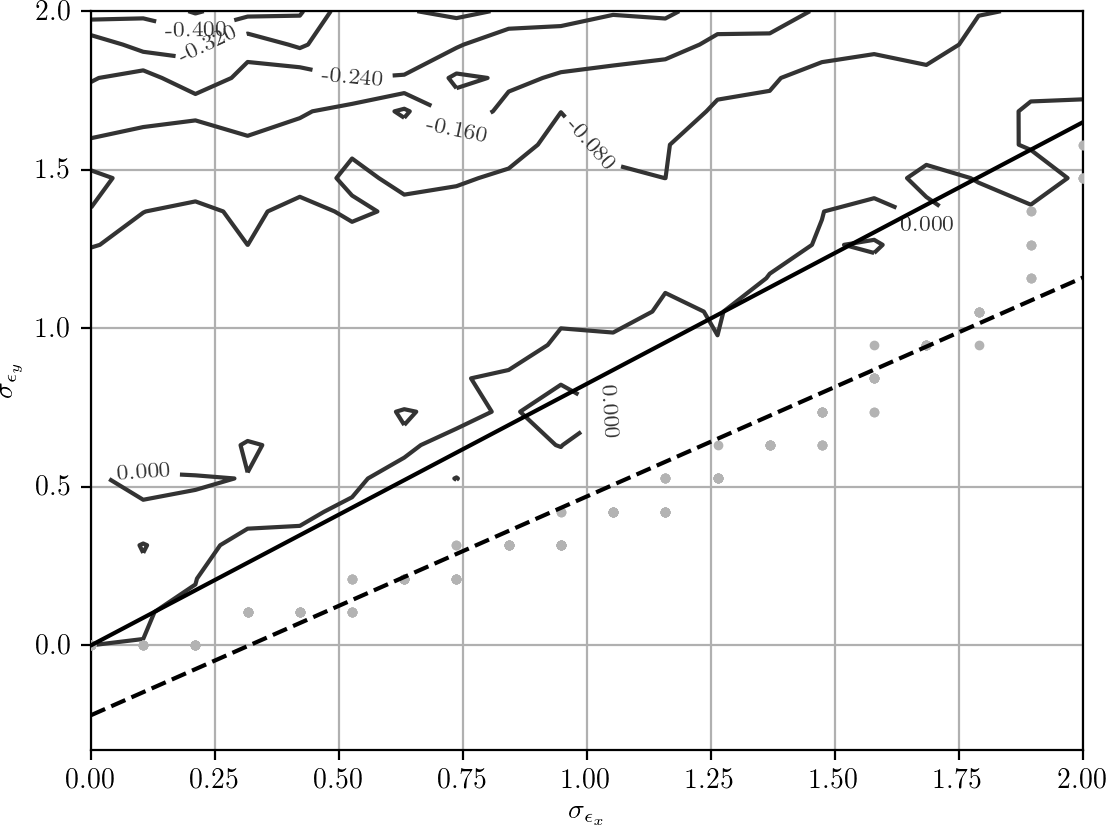
\includegraphics[width=135mm]{fig/linear/param/beta-0,125_param-accs-approx.png}
    \caption{\( \beta = 0{,}125 \)}
  \end{subfigure}

  \vspace{2\baselineskip}
  \begin{subfigure}[b]{\linewidth}
    \centering
    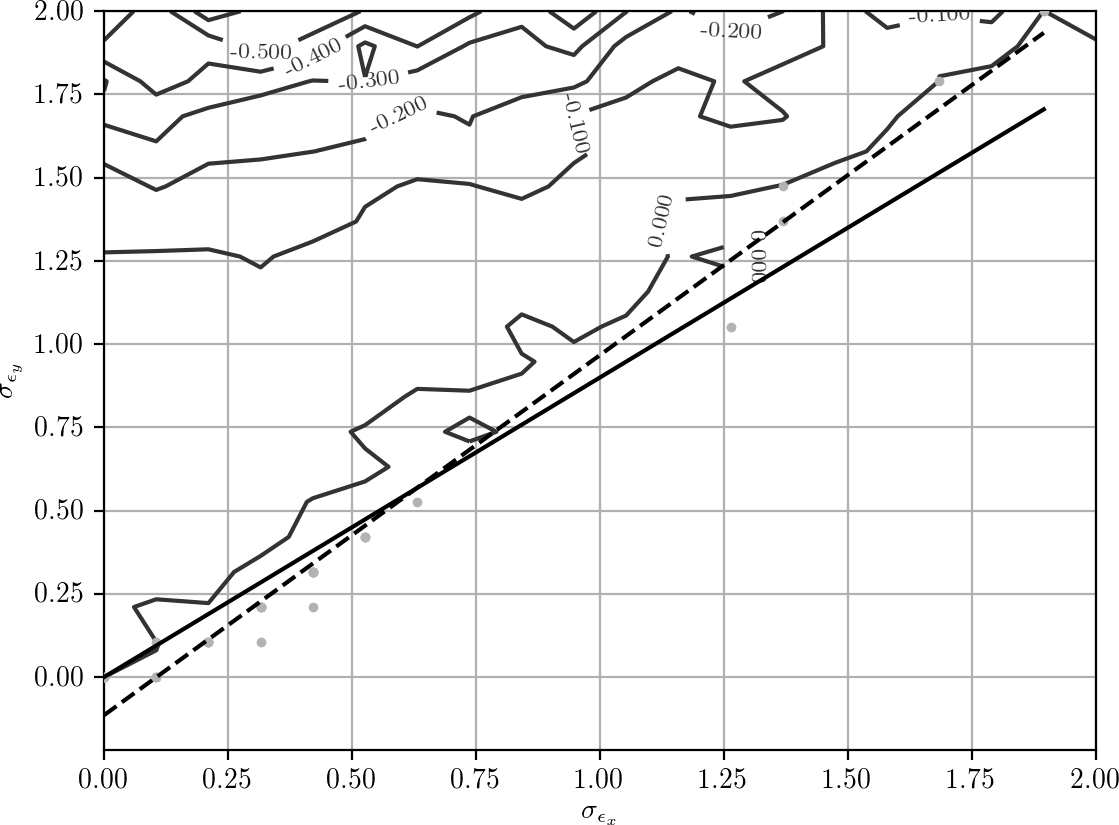
\includegraphics[width=135mm]{fig/linear/param/beta-0,2_param-accs-approx.png}
    \caption{\( \beta = 0{,}2 \)}
  \end{subfigure}

  \vspace{\baselineskip}
  \caption{%
    Сравнительная точность оценивания параметров \\
    линейных моделей с малыми коэффициентами усиления
  }\label{fig:comparison_linear_params_beta-small}
\end{figure}

При \( \beta = 0{,}5 \) (рисунок~\ref{fig:comparison_linear_params_beta-0,5}),
в случае, когда с.~к.~о ошибок наблюдений выхода системы превосходит
с.~к.~о ошибок наблюдений входа (\(\sigma_{\varepsilon_y} > 1{,}2 \sigma_{\varepsilon_x}\)),
МНК оценивает параметры системы более точно, чем МСА.
В противном случае МСА дает более точные оценки параметров.

\begin{figure}[h]
  \centering
  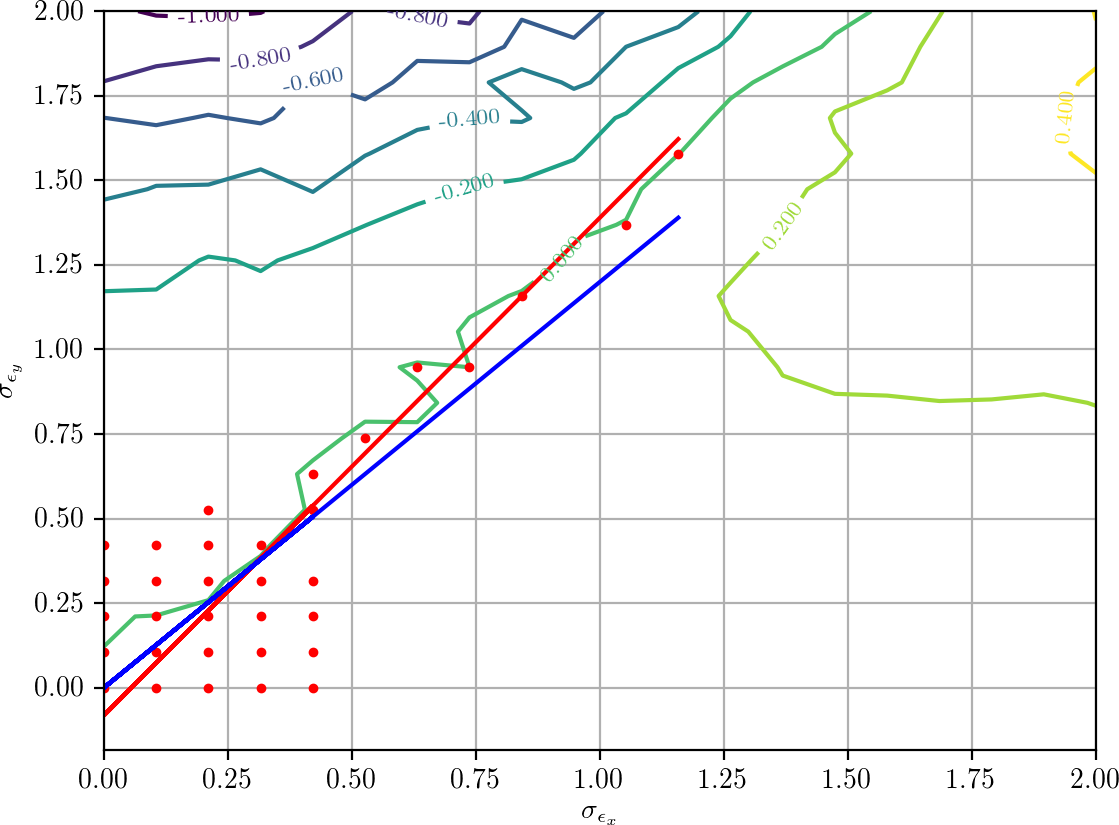
\includegraphics[width=135mm]{fig/linear/param/beta-0,5_param-accs-approx.png}
  \caption{%
    Сравнительная точность оценивания параметров \\
    линейной модели с коэффициентом усиления \( \beta = 0{,}5 \)
  }\label{fig:comparison_linear_params_beta-0,5}
\end{figure}

На рисунках~\ref{fig:comparison_linear_params_beta--1} и~\ref{fig:comparison_linear_params_beta-1}
представлены линии равного уровня зависимости \( d(\sigma_{\varepsilon_x}, \sigma_{\varepsilon_y}) \)
при \( \beta = -1 \) и \( \beta = 1 \).
Поскольку данные рисунки практически совпадают, можно утверждать, что точность рассматриваемых методов
зависит от абсолютного значения коэффициента усиления \( \beta \).

Из приведенных рисунков видно, что если с.~к.~о ошибок наблюдений выхода системы
более чем в полтора раза превосходит с.~к.~о ошибок наблюдений входа
(\( \sigma_{\varepsilon_y} > 1{,}7 \sigma_{\varepsilon_x} \)),
МНК оценивает параметры системы более точно, чем МСА.
В противном случае МСА дает более точные оценки параметров.

\begin{figure}[p]
  \begin{subfigure}[b]{\linewidth}
    \centering
    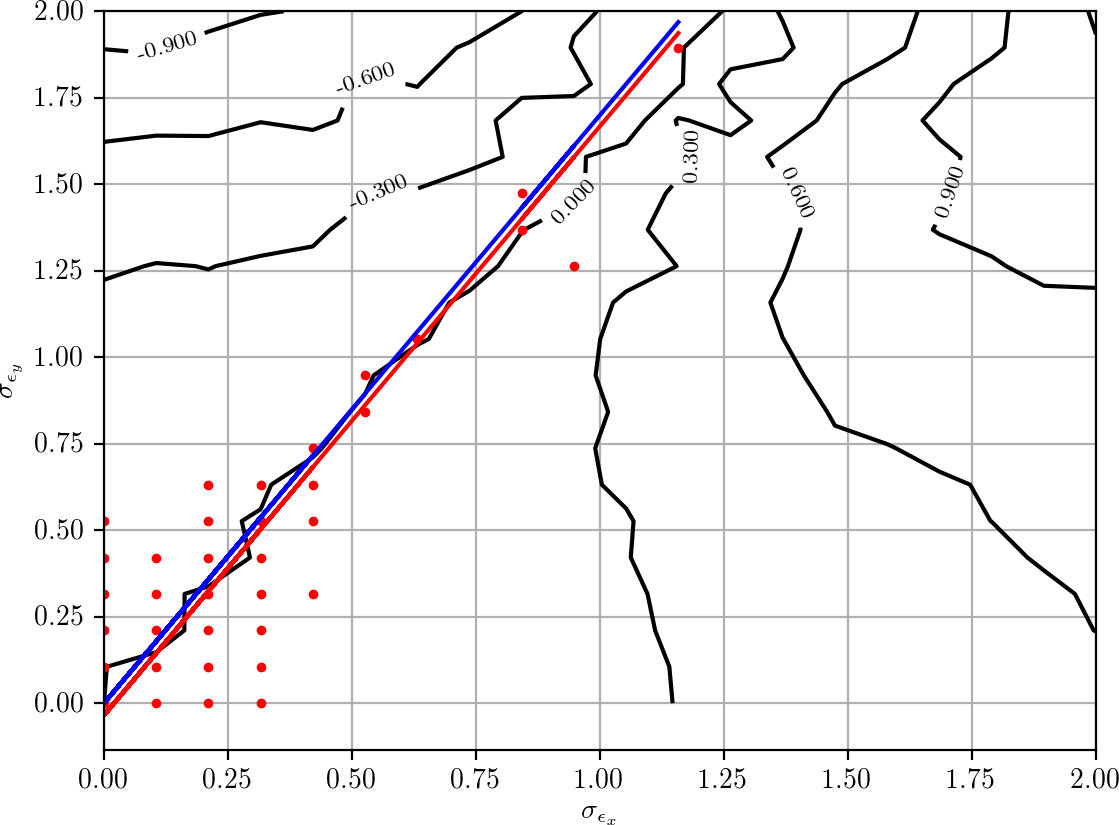
\includegraphics[width=135mm]{fig/linear/param/beta--1_param-accs-approx}
    \caption{\( \beta = -1 \)}\label{fig:comparison_linear_params_beta--1}
  \end{subfigure}

  \vspace{2\baselineskip}
  \begin{subfigure}[b]{\linewidth}
    \centering
    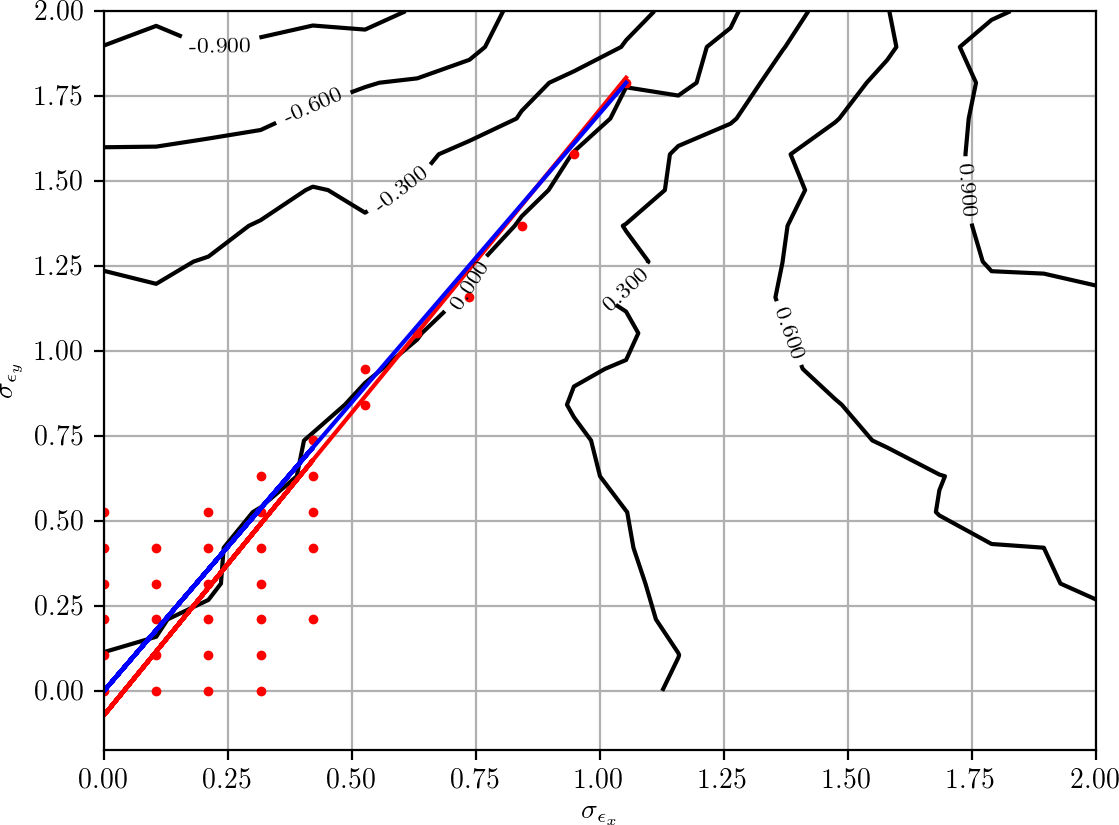
\includegraphics[width=135mm]{fig/linear/param/beta-1_param-accs-approx}
    \caption{\( \beta = 1 \)}\label{fig:comparison_linear_params_beta-1}
  \end{subfigure}

  \vspace{\baselineskip}
  \caption{%
    Сравнительная точность оценивания параметров \\
    линейных моделей с единичным коэффициентом усиления
  }\label{fig:comparison_linear_params_beta-one}
\end{figure}

\pagebreak
При \( \beta = 2 \) (рисунок~\ref{fig:comparison_linear_params_beta-2})
значение величины \( d \) зависит главным образом от значений с.~к.~о. ошибок
наблюдений входной переменной.
Если выполняется соотношение \( \sigma_{\varepsilon_y} > 2{,}7 \sigma_{\varepsilon_x} \),
то МНК оценивает ее параметры более точно, чем МСА.
В противном случае МСА дает более точные оценки параметров.

\begin{figure}[h]
  \centering
  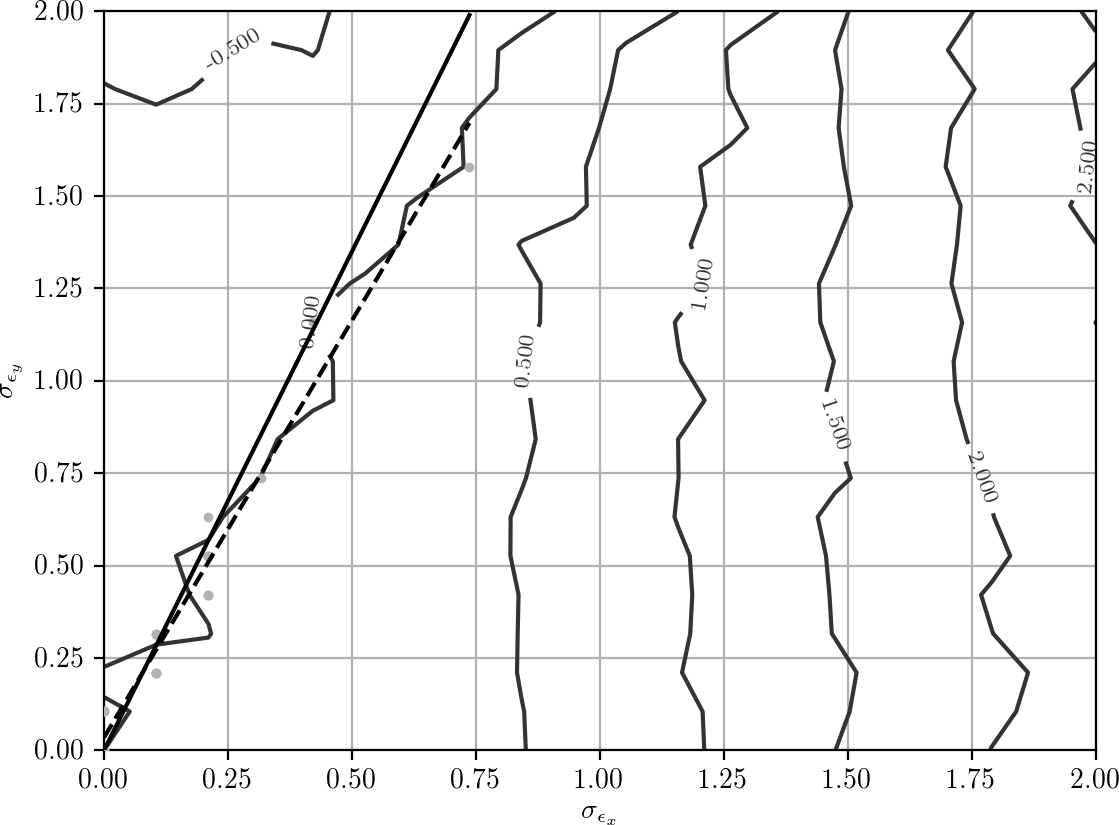
\includegraphics[width=135mm]{fig/linear/param/beta-2_param-accs-approx.png}
  \caption{%
    Сравнительная точность оценивания параметров \\
    линейной модели с коэффициентом усиления \( \beta = 2 \)
  }\label{fig:comparison_linear_params_beta-2}
\end{figure}

Данная тенденция усиливается при больших значениях коэффициента усиления модели
(рисунок~\ref{fig:comparison_linear_params_beta-big}).
При увеличении \( \sigma_{\varepsilon_y} \) относительно \( \sigma_{\varepsilon_x} \) значение
\( d \) быстро возрастает, что свидетельствует о том,
что при данных условиях МСА дает значительно более точные оценки параметров, чем МНК.

\begin{figure}[p]
  \begin{subfigure}[b]{\linewidth}
    \centering
    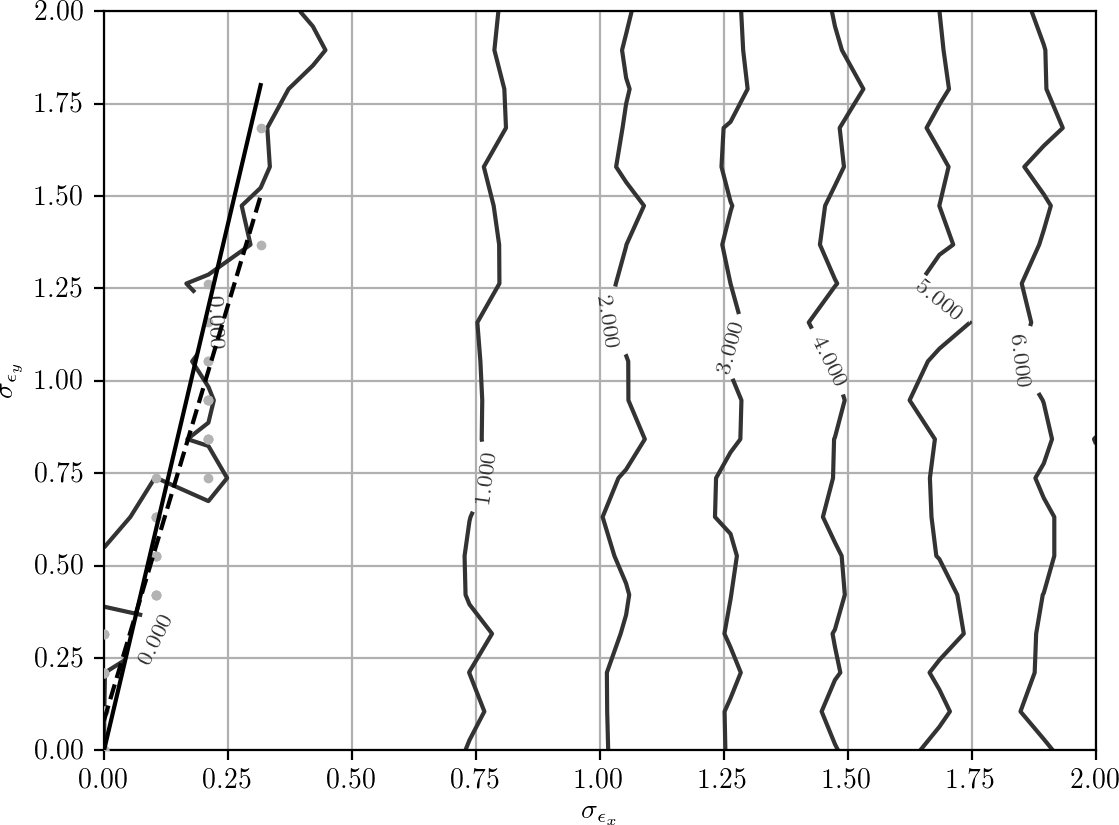
\includegraphics[width=135mm]{fig/linear/param/beta-5_param-accs-approx.png}
    \caption{\( \beta = 5 \)}
  \end{subfigure}

  \vspace{2\baselineskip}
  \begin{subfigure}[b]{\linewidth}
    \centering
    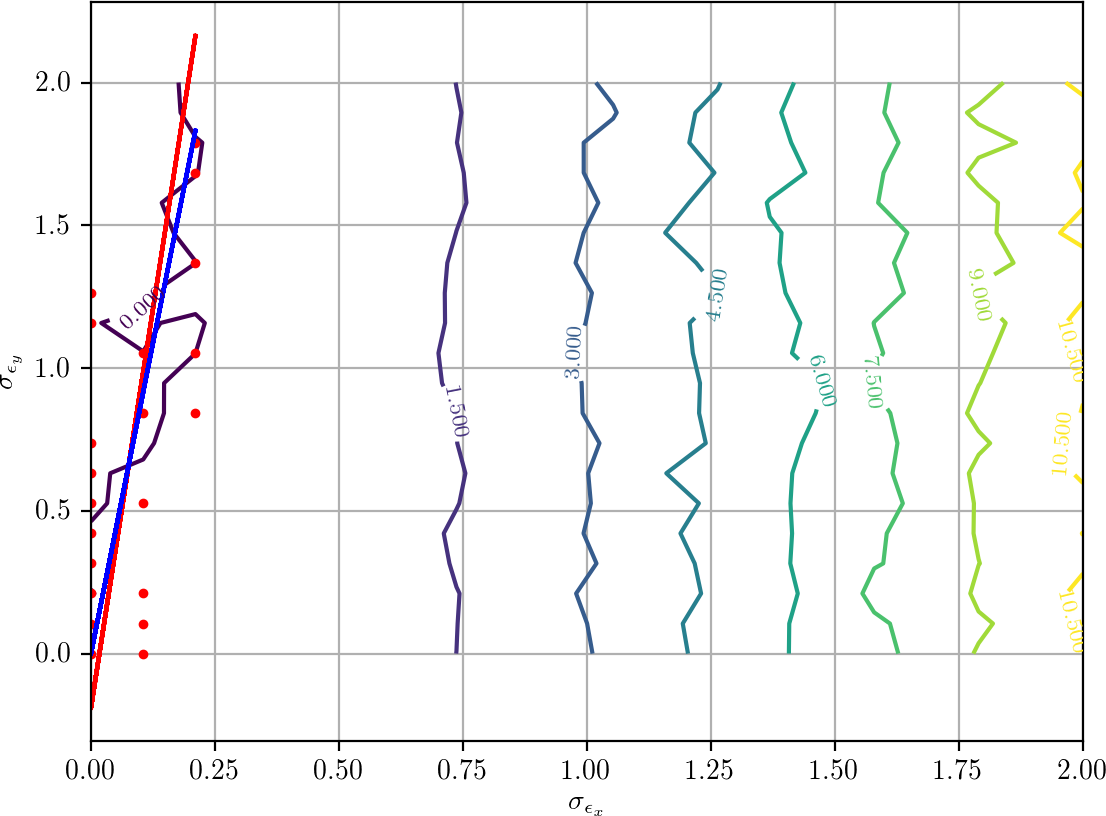
\includegraphics[width=135mm]{fig/linear/param/beta-8_param-accs-approx.png}
    \caption{\( \beta = 8 \)}
  \end{subfigure}

  \vspace{\baselineskip}
  \caption{%
    Сравнительная точность оценивания параметров \\
    линейных моделей с большими коэффициентами усиления
  }\label{fig:comparison_linear_params_beta-big}
\end{figure}

На основании изложенного можно сделать следуюшие выводы:
\begin{enumerate}
\item Точность оценивания параметров не зависит от фактического значения
  постоянной составляющей.
\item Точность оценивания параметров зависит от абсолютного значения
  коэффициента усиления системы и значений с.~к.~о. ошибок наблюдений
  входных и выходных переменных.
\item При больших значениях коэффициента усиления и с.~к.~о. ошибок наблюдений
  входных переменных метод симметричной аппроксимации оценивает
  параметры системы значительно точнее, чем метод наименьших квадратов.
\end{enumerate}

На основании результатов линейной аппроксимации линий нулевого уровня
зависимости величины \( d \) от с.~к.~о. ошибок входных и выходных наблюдений
\( \sigma_{\varepsilon_x}, \sigma_{\varepsilon_y} \)
при различных значениях коэффициента усиления \( \beta \) предлагается использовать
следующую эмпирическую зависимость для принятия решения о том, какой метод
использовать более предпочтительно: \\
<<Если условие
\begin{equation}
  \sigma_{\varepsilon_y} > (0{,}7 + |\beta|) \sigma_{\varepsilon_x}
  \label{eq:linear_rule_param}
\end{equation}
выполняется, то метод наименьших квадратов оценивает параметры линейной
стохастической системы второго типа более точно, чем метод симметричной аппроксимации.
В противном случае метод симметричной аппроксимации позволяет получить
оценки более высокой точности, чем метод наименьших квадратов>>.

\subsection{Точность прогнозирования наблюдений выхода}

Было выполнено сравнение точности прогнозирования наблюдений выхода по
наблюдениям входа системы~\eqref{eq:linear_model_scalar} на основании оценок параметров,
полученными методом наименьших квадратов и методом симметричной аппроксимации,
в зависимости от c.~к.~о. ошибок наблюдений \( \sigma_{\varepsilon_x}, \sigma_{\varepsilon_y} \).

В качестве величины, характеризующей точность прогнозирования,
использовалась разность средних Евклидовых расстояний между наблюдениями выхода модели и
их оценками, полученными МНК и МСА:
\begin{equation*}
  \begin{aligned}
    d &= d_{\text{МНК}} - d_{\text{МСА}}, \\
    d_{\text{МНК}} &= \frac{1}{k} \sum_{j=1}^k \sqrt{ \sum_{i=1}^n (\hat{\alpha}_{\text{МНК}_j} + \hat{\beta}_{\text{МНК}_j} x_{ij} - y_{ij})^2}, \\
    d_{\text{МСА}} &= \frac{1}{k} \sum_{j=1}^k \sqrt{ \sum_{i=1}^n (\hat{\alpha}_{\text{МСА}_j} + \hat{\beta}_{\text{МСА}_j} x_{ij} - y_{ij})^2},
    \end{aligned}
  \end{equation*}
где \( k \) --- число оценок.

Расчеты расстояний \( d \) производились в узлах сетки значений
\( \sigma_{\varepsilon_x}, \sigma_{\varepsilon_y} \) в прямоугольнике
\( [0, 2] \times [0, 2] \) с шагом 0{,}1.
В каждом узле сетки вычислялось сто оценок (\( k = 100 \)).
Для получения каждой оценки \( \hat{\alpha}, \hat{\beta} \) использовались результаты
ста наблюдений \( ( x_i, y_i ), i = \overline{1, n}, n = 100 \).

На рисунках~\ref{fig:comparison_linear_predict_beta-0,2}--\ref{fig:comparison_linear_predict_beta-5}
представлены линии равного уровня зависимости \( d(\sigma_{\varepsilon_x}, \sigma_{\varepsilon_y}) \)
при различных значениях коэффициента усиления модели \( \beta \).
Отрицательные значения величины \( d \) свидетельствуют о том,
что точность прогнозирования значений выхода с помощью МСА при данных с.~к.~о.
ошибок наблюдений превосходит точность МНК,
а положительные говорят о том, что в данных условиях прогнозы, полученные с помощью МНК,
являются более точными.
При \( d = 0 \) сравниваемые методы прогнозируют наблюдения выхода системы с
равной точностью.

Поскольку на приведенных рисунках величина \( d \) не принимает положительных значений,
можно сделать вывод, что метод наименьших квадратов дает более точные оценки
наблюдений выхода по наблюдениям входа системы, чем метод симметричной аппроксимации
на всем рассмотренном множестве значений коэффициента усиления и с.~к.~о. ошибок наблюдений.

\begin{figure}[h]
  \centering
  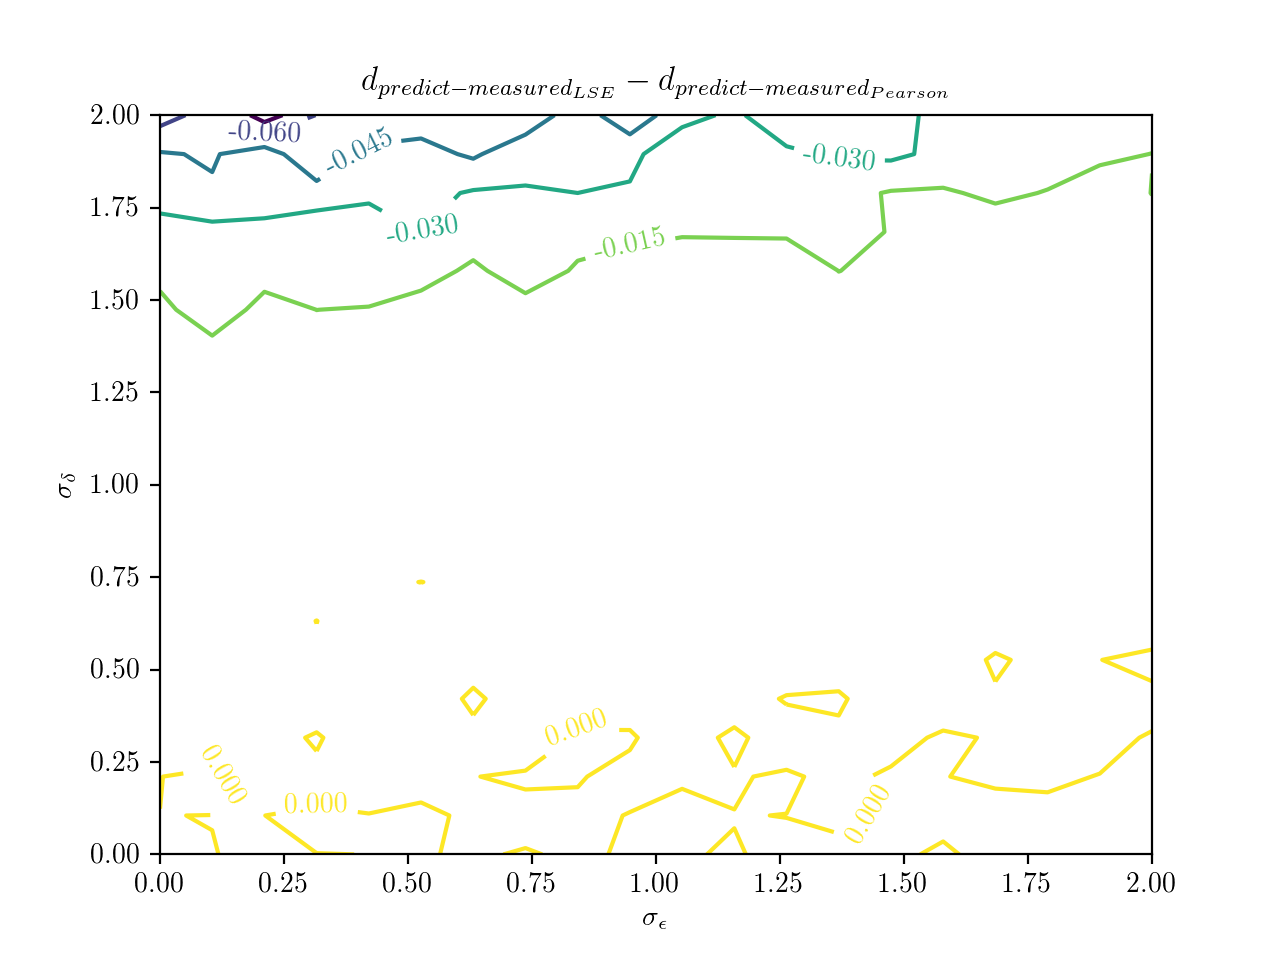
\includegraphics[width=135mm]{fig/linear/predict/beta-0,2_predict-measured.png}
  \caption{%
    Сравнительная точность прогнозирования наблюдений \\
    выхода линейной модели с коэффициентом усиления \( \beta = 0{,}2 \)
  }\label{fig:comparison_linear_predict_beta-0,2}
\end{figure}

\begin{figure}[p]
  \centering
  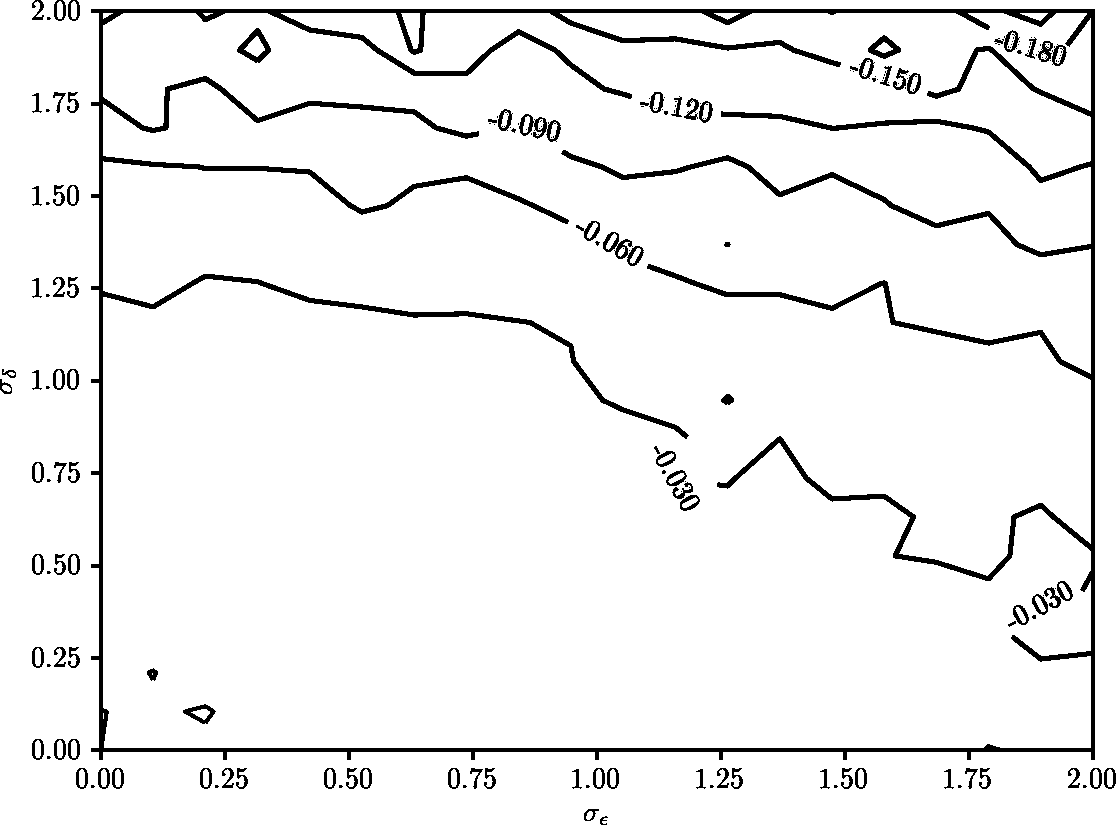
\includegraphics[width=135mm]{fig/linear/predict/beta-1_predict-measured.png}
  \caption{%
    Сравнительная точность прогнозирования наблюдений \\
    выхода линейной модели с коэффициентом усиления \( \beta = 1 \)
  }\label{fig:comparison_linear_predict_beta-1}
\end{figure}

\begin{figure}[p]
  \centering
  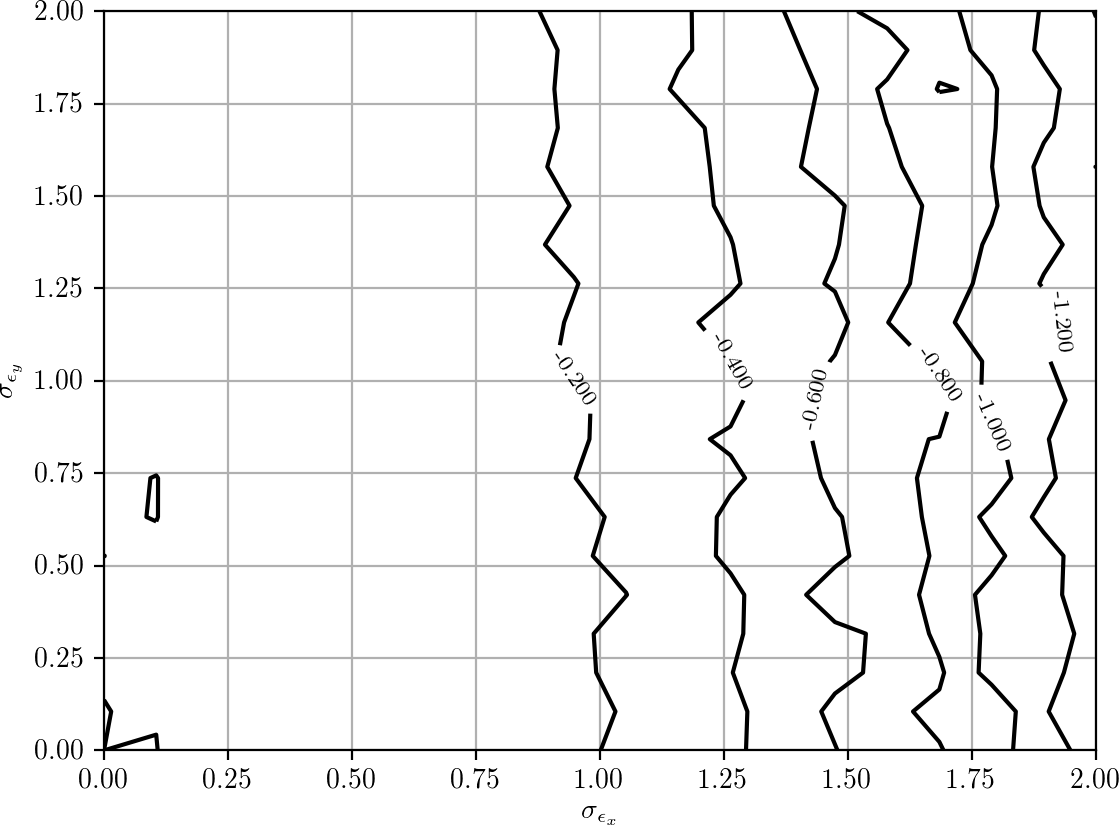
\includegraphics[width=135mm]{fig/linear/predict/beta-5_predict-measured.png}
  \caption{%
    Сравнительная точность прогнозирования наблюдений \\
    выхода линейной модели с коэффициентом усиления \( \beta = 5 \)
  }\label{fig:comparison_linear_predict_beta-5}
\end{figure}

\section{Выводы}

\begin{enumerate}
\item Разработаны алгоритмы и программные реализации классического
  метода наименьших квадратов и метода симметричной аппроксимации.
\item Выполнен численный анализ точности оценивания параметров и
  прогнозирования наблюдений выхода по наблюдениям входа линейных
  стохастических систем второго типа.
\item На основании результатов анализа получена эмпирическая зависимость
  для выбора более точного метода оценивания параметров линейных стохастических
  систем второго типа.
\end{enumerate}
